\chapter{Learning Methods}


Throughout this section, we'll be doing an in-depth description of the full guidance, navigation, control, and learning architecture which was used during this work. While reading the following subsections, please refer back to figure \ref{fig:Training_Flowchart}, which offers a compact visualization of the whole training loop:


\begin{figure}[H]
    \centering
    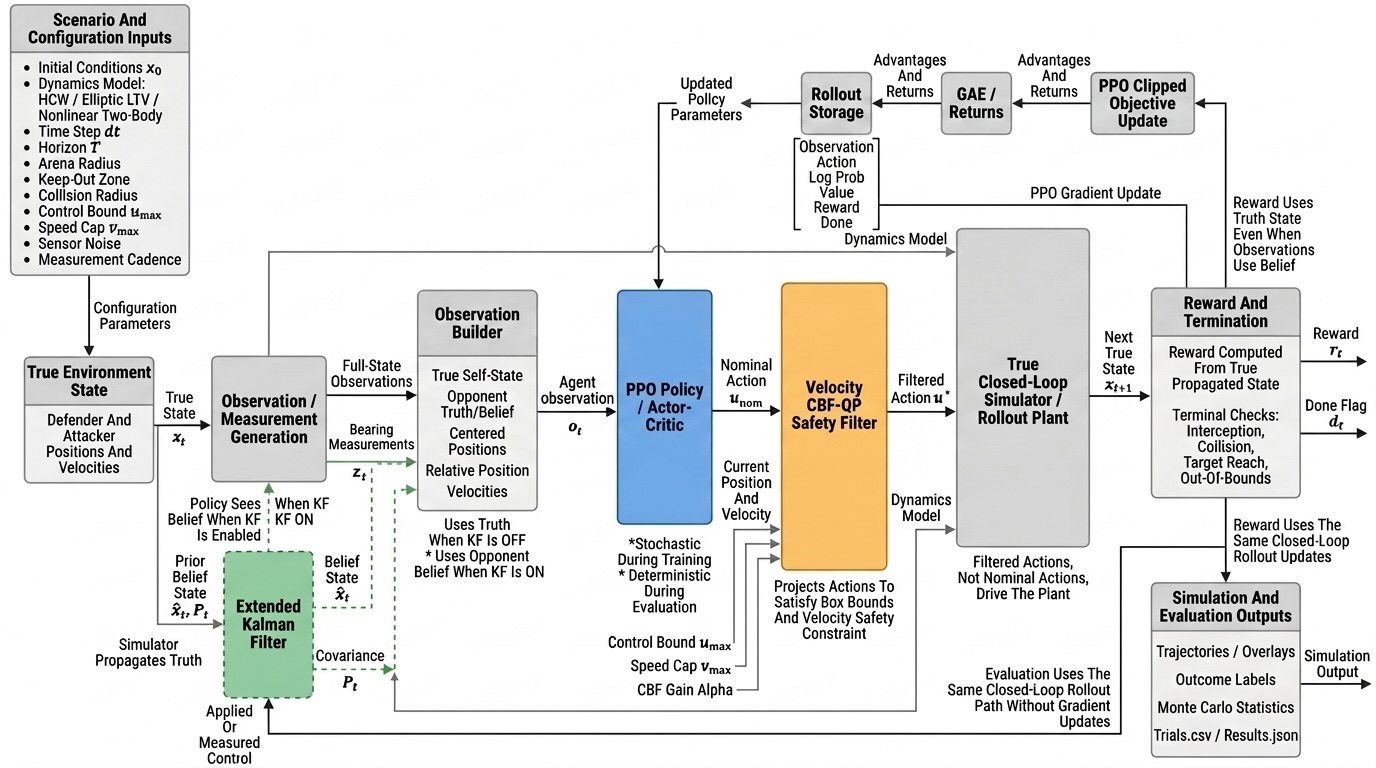
\includegraphics[width=1.0\linewidth]{Figures/Training_Improved_Flattened.jpg}
    \caption{Diagram showing the PARL + BC algorithm's learning loop within the GNC architecture constrained by the Extended Kalman Filter and the Classical CBF-QP controller}
    \label{fig:Training_Flowchart}
\end{figure}


\section{Single Phase PPO Algorithm}
\label{sec:single-phase-ppo}

We collect on-policy results via the PPO algorithm, based on the foundational work by \cite{schulman2017ppo} and adapted to our dynamics and environment models, where the batches are a fixed length from \(N\) vectorized environments, each of length \(H\), and hence yielding \(B=NH\) transitions per update on each policy. Algorithm \ref{alg:ppo_full_obs} describes the single phase PPO training with full-state observations, whereas algorithm \ref{alg:ppo_kf_on} describes the modifications that are made to the latter when doing partial observability trainings with the bearings-only EKF measurements: 


\begin{algorithm}[H]
\caption{Single-Phase PPO Update with Full-State Observations}
\label{alg:ppo_full_obs}
\begin{algorithmic}[1]
\Require Learning role $r\in\{\textsc{def},\textsc{att}\}$, fixed opponent controller $\Pi_{\bar r}$, horizon $H$, vectorized environments $N$
\Require Full-state observation maps $\mathrm{Obs}^{\mathrm{full}}_r,\mathrm{Obs}^{\mathrm{full}}_{\bar r}$, dynamics $\mathcal{D}(\cdot)$, reward $\mathcal{R}(\cdot)$
\Ensure Updated policy parameters $\theta_r$

\State \textbf{Initialize vectorized PPO training:}
\State \hspace{1em} Initialize VecEnv($N$), configured dynamics, learning policy $\pi_{\theta_r}$, and value function $V_{\theta_r}$

\For{$u=1,\dots,U$}
  \State \textbf{Prepare a new rollout batch:}
  \State \hspace{1em} Optionally decay learning rate and anneal environment coefficients
  \State \hspace{1em} Initialize rollout buffer $\mathcal{B}_r$

  \For{$t=1,\dots,H$ \textbf{in parallel over} $n=1,\dots,N$}
    \State \textbf{Build full-state observations:}
    \State \hspace{1em} $\vec{\mathbf{o}}_t^{r,(n)} \leftarrow \mathrm{Obs}^{\mathrm{full}}_r(\vec{\mathbf{x}}_t^{(n)})$
    \State \hspace{1em} $\vec{\mathbf{o}}_t^{\bar r,(n)} \leftarrow \mathrm{Obs}^{\mathrm{full}}_{\bar r}(\vec{\mathbf{x}}_t^{(n)})$

    \State \textbf{Select learner and opponent actions:}
    \State \hspace{1em} $\vec{\mathbf{a}}_t^{r,(n)} \sim \pi_{\theta_r}(\cdot \mid \vec{\mathbf{o}}_t^{r,(n)})$
    \State \hspace{1em} $\vec{\mathbf{a}}_t^{\bar r,(n)} \leftarrow \Pi_{\bar r}(\vec{\mathbf{o}}_t^{\bar r,(n)})$
    \Comment{rule-based or deterministic frozen RL policy}

    \State \textbf{Step the environment:}
    \State \hspace{1em} $(\vec{\mathbf{o}}_{t+1}^{r,(n)}, r_t^{r,(n)}, d_t^{(n)}) \leftarrow \textsc{Step}(\vec{\mathbf{a}}_t^{r,(n)}, \vec{\mathbf{a}}_t^{\bar r,(n)})$

    \State \textbf{Conceptually, this step entails:}
    \State \hspace{2em} $\vec{\mathbf{x}}_{t+1}^{(n)} \leftarrow \mathcal{D}\!\left(\vec{\mathbf{x}}_t^{(n)}, \vec{\mathbf{a}}_t^{r,(n)}, \vec{\mathbf{a}}_t^{\bar r,(n)}\right)$
    \Comment{propagate the true spacecraft state}
    \State \hspace{2em} $r_t^{r,(n)} \leftarrow \mathcal{R}\!\left(\vec{\mathbf{x}}_{t+1}^{(n)}, \vec{\mathbf{a}}_t^{r,(n)}, \vec{\mathbf{a}}_t^{\bar r,(n)}\right)$
    \Comment{evaluate the role-specific reward from the realized transition}
    \State \hspace{2em} $d_t^{(n)} \leftarrow \mathrm{Done}\!\left(\vec{\mathbf{x}}_{t+1}^{(n)}\right)$
    \Comment{check terminal conditions such as docking, interception, or boundary violation}
    \State \hspace{2em} $\vec{\mathbf{o}}_{t+1}^{r,(n)} \leftarrow \mathrm{Obs}^{\mathrm{full}}_r(\vec{\mathbf{x}}_{t+1}^{(n)})$
    \Comment{form the next observation from the updated true state}

    \State \textbf{Store the rollout transition:}
    \State \hspace{1em} Store $\big(\vec{\mathbf{o}}_t^{r,(n)}, \vec{\mathbf{a}}_t^{r,(n)}, \log \pi_{\theta_r}, V_{\theta_r}, r_t^{r,(n)}, d_t^{(n)}\big)$ in $\mathcal{B}_r$
    \Comment{terminated environments are reset internally in the vectorized implementation}
  \EndFor

  \State \textbf{Compute returns and advantages from rewards:}
  \State \hspace{1em} Bootstrap $V_{\theta_r}(\vec{\mathbf{o}}_{H+1}^r)$
  \State \hspace{1em} Compute done-masked returns and GAE advantages from the stored rewards

  \State \textbf{Update the policy and value function with PPO:}
  \State \hspace{1em} Normalize advantages and optimize the PPO clipped surrogate objective
  \State \hspace{1em} using policy loss, value loss, and entropy regularization for $E$ epochs
\EndFor
\end{algorithmic}
\end{algorithm}

\begin{algorithm}[H]
\caption{KF-On Modifications to Algorithm \ref{alg:ppo_full_obs}}
\label{alg:ppo_kf_on}
\begin{algorithmic}[1]
\Require Estimator $\mathcal{E}$ with belief state $\hat{\vec{\mathbf{x}}}_t$ and measurement model $\vec{\mathbf{y}}_t$

\State Run Algorithm \ref{alg:ppo_full_obs} unchanged, except replace the observation/reward portion of each rollout step by the following:

\State \textbf{Maintain both truth and belief:}
\State \hspace{1em} The simulator propagates the true state $\vec{\mathbf{x}}_t$, while the policy receives observations derived from the estimator state $\hat{\vec{\mathbf{x}}}_t$

\State \textbf{Build estimator-based observations:}
\State \hspace{1em} $\vec{\mathbf{o}}_t^r \leftarrow \mathrm{Obs}^{\mathrm{KF}}_r(\vec{\mathbf{x}}_t,\hat{\vec{\mathbf{x}}}_t)$
\State \hspace{1em} $\vec{\mathbf{o}}_t^{\bar r} \leftarrow \mathrm{Obs}^{\mathrm{KF}}_{\bar r}(\vec{\mathbf{x}}_t,\hat{\vec{\mathbf{x}}}_t)$
\Comment{Opponent-state entries are replaced by estimator beliefs when not directly observed}

\State \textbf{Select actions exactly as in Algorithm \ref{alg:ppo_full_obs}}

\State \textbf{Propagate truth, then update the estimator:}
\State \hspace{1em} $\vec{\mathbf{x}}_{t+1} \leftarrow \mathcal{D}(\vec{\mathbf{x}}_t,\vec{\mathbf{a}}_t^r,\vec{\mathbf{a}}_t^{\bar r})$
\State \hspace{1em} $\hat{\vec{\mathbf{x}}}_{t+1} \leftarrow \mathcal{E}(\hat{\vec{\mathbf{x}}}_t,\vec{\mathbf{a}}_t^r,\vec{\mathbf{a}}_t^{\bar r},\vec{\mathbf{y}}_{t+1})$

\State \textbf{Compute reward from the true state:}
\State \hspace{1em} $r_t^r \leftarrow \mathcal{R}(\vec{\mathbf{x}}_{t+1},\vec{\mathbf{a}}_t^r,\vec{\mathbf{a}}_t^{\bar r})$
\Comment{Current KF-on training still uses true-state reward geometry}

\State \textbf{Store the estimator-based observation in the rollout buffer, then continue with bootstrap, GAE, and PPO updates exactly as in Algorithm \ref{alg:ppo_full_obs}}
\end{algorithmic}
\end{algorithm}


\subsection{Policy development}
\label{subsec:policy-development}


Given an observation \(\vec{\mathbf{o}}\) (equations \ref{eq:Full_Obs_Both_Agents}, \ref{eq:EKF_Obs_Agent_1}, and \ref{eq:EKF_Obs_Agent_2}), we obtain an action $\vec{\boldsymbol{\mu}}(\vec{\mathbf{o}})$ for the queried role \(\mathrm{who}\in\{\mathrm{def},\mathrm{att}\}\). From there, the action is sampled from a factorized normal distribution and squashed to enforce the actuation bound:

\[
\vec{\mathbf{u}}_{raw} \sim \mathcal{N}\!\left(\vec{\boldsymbol{\mu}}(\vec{\mathbf{o}}),\, \operatorname{diag}\!\left(\vec{\boldsymbol{\sigma}}^{\,2}\right)\right),
\qquad
\vec{\mathbf{a}} = u_{\max}\tanh\!\left(\vec{\mathbf{u}}_{raw}\right).
\]

From there, the corrected log-probability for PPO is
\[
\log \pi(\vec{\mathbf{a}} \mid \vec{\mathbf{o}})
=
\log \mathcal{N}\!\left(\vec{\mathbf{u}}_{raw};\, \vec{\boldsymbol{\mu}},\, \vec{\boldsymbol{\sigma}}^{\,2}\right)
-
\sum_{j=1}^{D}\log\!\left(1-\tanh^2(u_{raw,j})\right).
\]


The critic \(V_\theta(\vec{\mathbf{o}})\) then maps the full observation \(\vec{\mathbf{o}}\) to a scalar value estimate used in the advantage and return calculations during PPO updates.



\subsection{Advantage Estimation and PPO Objective}
\label{subsec:advantage-estimation-ppo}
We use generalized advantage estimation (GAE) in the following form:
\[
\begin{aligned}
\delta_t \;&= r_t + \gamma(1-d_t)\,V(\vec{\mathbf{o}}_{t+1}) - V(\vec{\mathbf{o}}_{t}),\\[4pt]
A_t \;&= \sum_{l=0}^{\infty} (\gamma\lambda)^l
\left(\prod_{k=1}^{l} (1-d_{t+k})\right)\delta_{t+l}.
\end{aligned}
\]

with terminal flags \(d_t\in\{0,1\}\). Letting  \(R_t=A_t+V(\vec{\mathbf{o}}_t)\) for a minibatch \(\mathcal{B}\), the PPO maximizes the training objective:
\begin{align*}
\mathcal{L}_{\text{PPO}}
&= \mathbb{E}_{\mathcal{B}}\Big[
\min\!\big(r_t A_t,\ \mathrm{clip}(r_t,\,1{-}\epsilon,\,1{+}\epsilon)\,A_t\big)
\\
&\quad -\, c_v\,\underbrace{\big(V(\vec{\mathbf{o}}_t) - R_t\big)^2}_{\text{(with value clipping)}}
\;+\; c_{\mathcal{H}}\,\mathcal{H}\!\big[\pi(\cdot\!\mid \vec{\mathbf{o}}_t)\big]
\Big],
\end{align*}

where \(r_t=\exp\!\left(\log\pi_\theta(\vec{\mathbf{a}}_t \mid \vec{\mathbf{o}}_t)-\log\pi_{\mathrm{old}}(\vec{\mathbf{a}}_t \mid \vec{\mathbf{o}}_t)\right)\),
\(\epsilon\) is the policy clip, and \(c_v,c_{\mathcal{H}}>0\) weight the value loss and entropy bonus, while applying global gradient clipping and standard Adam optimizers.


\section{Phased Stationary Training Schedule}
\label{sec:phased-stationary-training}

The process described in algorithm \ref{alg:ppo_full_obs} (and the KF specifics from algorithm \ref{alg:ppo_kf_on}) is then replicated in independent phases of training. Following a 0th phase where the defender is trained interchangeably against a rule-based attacker to warm-start the training, each attacker or defender policy is trained against a combination of the resulting trained defender or attacker policies from previous phases. This process is called domain randomization, where training the agents against different versions of their opponents allows for the progressive development of sequentially stronger and smarter defender and attacker policies. By training against multiple policies at once, we mitigate overfitting to any one policy, one of the core issues of RL algorithms as described in the introduction. Therefore, this allows for the creation of smarter, more generalizable policies for the attacker and defender. Algorithm \ref{alg:ppo_phases} describes the phased training schedule.



\begin{algorithm}[H]
\caption{Phased Alternating Training Cycle with Opponent Randomization}
\label{alg:ppo_phases}
\begin{algorithmic}[1]
\State \textbf{Phase 0: Train defender teacher $\pi_{def,0}$ against the rule-based attacker:}
\State \hspace{1em} Build cfg with $\texttt{attacker\_mode}=\textsc{rule}$ and $\texttt{train\_role}=\textsc{def}$
\State \hspace{1em} Do not use a checkpoint-based opponent mixture in this phase
\State \hspace{1em} Train the defender teacher and retain checkpoint $\theta_{D0}$

\State \textbf{Phase 1: Train attacker teacher $\pi_{att,1}$ against a frozen defender mixture based on $\pi_{def,0}$:}
\State \hspace{1em} Build cfg with $\texttt{attacker\_mode}=\textsc{rl}$ and $\texttt{train\_role}=\textsc{att}$
\State \hspace{1em} Load $\theta_{D0}$ and freeze defender parameters
\State \hspace{1em} Define opponent variants from the same frozen defender checkpoint:
\Statex \hspace{2em} full: $(\texttt{action\_scale},\texttt{noise\_std})=(1.0,0.0)$
\Statex \hspace{2em} weak: $(0.25,0.05)$
\Statex \hspace{2em} very-weak: $(0.0,0.0)$
\State \hspace{1em} Set
\Statex \hspace{2em}
$\texttt{opp\_mix}\gets\{(\pi_{def,0}^{\text{full}},0.5),(\pi_{def,0}^{\text{weak}},0.3),(\pi_{def,0}^{\text{very\mbox{-}weak}},0.2)\}$
\State \hspace{1em} Resample the active opponent variant from $\texttt{opp\_mix}$ at each episode
\State \hspace{1em} Train the attacker teacher and retain checkpoint $\theta_{A1}$

\State \textbf{Phase 2: Fine-tune defender teacher $\pi_{def,0}\!\rightarrow\!\pi_{def,1}$ against a frozen attacker mixture based on $\pi_{att,1}$:}
\State \hspace{1em} Build cfg with $\texttt{attacker\_mode}=\textsc{rl}$ and $\texttt{train\_role}=\textsc{def}$
\State \hspace{1em} Load $\theta_{D0}$ as the defender initialization
\State \hspace{1em} Load $\theta_{A1}$ and freeze attacker parameters
\State \hspace{1em} Define opponent variants from the same frozen attacker checkpoint:
\Statex \hspace{2em} full: $(\texttt{action\_scale},\texttt{noise\_std})=(1.0,0.0)$
\Statex \hspace{2em} weak: $(0.25,0.05)$
\Statex \hspace{2em} very-weak: $(0.0,0.0)$
\State \hspace{1em} Set
\Statex \hspace{2em}
$\texttt{opp\_mix}\gets\{(\pi_{att,1}^{\text{full}},0.5),(\pi_{att,1}^{\text{weak}},0.3),(\pi_{att,1}^{\text{very\mbox{-}weak}},0.2)\}$
\State \hspace{1em} Resample the active opponent variant from $\texttt{opp\_mix}$ at each episode
\State \hspace{1em} Train the defender teacher and retain checkpoint $\theta_{D1}$
\State \textbf{Continue the alternating procedure for subsequent phases:}
\State \hspace{1em} Repeat the same attacker-training and defender-training pattern with the most recent frozen opponent checkpoint(s) and the corresponding checkpoint-based opponent mixture until the final scheduled phase is reached (Phase 3 trains $\pi_{att,2}$ and Phase 4 trains $\pi_{def,2}$, yielding five phases total including Phase 0)
\end{algorithmic}
\end{algorithm}


Most importantly though, by freezing the opposing policy on each training phase we ensure the stationarity of the Markov chain in the decision process during learning. Other published methods on zero-sum games attempt to skip this phased approach in favor of a simultaneous self-play method, where both agents train their policies at once and learn within the same phase using entropy regularization methods, such as that of \cite{rudolph2025reevaluating}, but these methods tend to be unstable in certain contexts. In fact, we unsuccessfully attempted to do a similar simultaneous self-play approach in this context in the earlier stages of this research, and unfavorable results were what led us to pursue this phased stationary method.

Other approaches that we experimented with were the use of residual networks with Nash differentials or classical controller priors, which could be a potential future direction for this work. Nevertheless, we found that skipping residual networks and giving full power to PPO to carry on with the optimization ended up being much simpler to iterate on and interpret results for.

\subsection{Rule-Based Attacker for phase 0 defender warm start}
\label{subsec:rule-based-attacker-warm-start}
To warm start the training, the attacker control input in the initial warm-up phase (phase 0) is not defined by a PPO policy, but rather by an arbitrary, saturated convex combination with predefined weights.

First we obtain $\vec{\mathbf{u}}_{\text{center}}$, a one-step ridge least-squares action that pulls \(\vec{\mathbf{p}}_2\) towards \(\vec{\mathbf{c}}\) (the asset/object of interest). Considering the position projection (\(P=[I\ \ 0]\in\mathbb{R}^{D\times 2D}\) ), the next-step position error (\(\vec{\mathbf{E}}_2:= P A_d \vec{\mathbf{x}}_2 - \vec{\mathbf{c}}\), given \(\vec{\mathbf{x}}_2=\begin{bmatrix}\vec{\mathbf{p}}_2\\ \vec{\mathbf{v}}_2\end{bmatrix}\)), and the position influence matrix (\(F := P B_d \in\mathbb{R}^{D\times D}\)), we obtain the least-squares solution, so that $\vec{\mathbf{u}}_{\text{center}}$ takes the form:

\[
\vec{\mathbf{u}}_{\text{center}} \;=\; - K\,\vec{\mathbf{E}}_2,\qquad
K \;=\; (F^\top F + \lambda I)^{-1} F^\top
\],

To this we add \(\vec{\mathbf{u}}_{\text{repulse}}\), a term that is meant to push the attacker away from the defender. Considering \(\vec{\mathbf{r}} := \vec{\mathbf{p}}_2-\vec{\mathbf{p}}_1\), \(r_{\min}>0\), gain \(g>0\), and a small term \(\varepsilon > 0\) that prevents the expression from blowing up at 0, \(\vec{\mathbf{u}}_{\text{repulse}}\) is defined as:
\[
\vec{\mathbf{u}}_{\text{repulse}} \;=\; \frac{g}{\big(\max\{r_{\min}^2,\ \|\vec{\mathbf{r}}\|^2\}+\varepsilon\big)^{3/2}}\; \vec{\mathbf{r}}.
\]

In addition to the two terms described before, we add a small penalty for the attacker velocity \(\vec{\mathbf{v}}_2\).


Then we add these terms together, with proper weights $w_c$, $w_r$, and $w_d$ for each, into a final acceleration that is saturated relative to the max actuation limit:


\[
\boxed{
\vec{\mathbf{u}}_2 \;=\; \operatorname{sat}_{u_{\max}}\!\left(
w_c\,\vec{\mathbf{u}}_{\text{center}} + w_r\,\vec{\mathbf{u}}_{\text{repulse}} - w_d\,\vec{\mathbf{v}}_2\right)},
\]











\section{Inference.}
\label{sec:inference}
At inference during policy evaluation, we translate observations into actuator commands that can be used by the spacecraft relative to a bounded commanded acceleration. At evaluation time we use the same 5D observation vectors as described in \ref{eq:Full_Obs_Both_Agents}, \ref{eq:EKF_Obs_Agent_1}, or \ref{eq:EKF_Obs_Agent_2}, depending on the case.

By default we run a deterministic evaluation, \(\vec{\mathbf{u}}_t^{\mathrm{raw}}=\vec{\boldsymbol{\mu}}_\theta(\vec{\mathbf{o}}_t)\), where actions come from a squashed-Gaussian actor to guarantee that \(\|\vec{\mathbf{u}}_t^{\mathrm{cmd}}\|_\infty \le u_{\max}\). When we report stochastic results, we instead sample \(\vec{\mathbf{u}}_t^{\mathrm{raw}}\) from the diagonal Gaussian policy and then apply tanh squashing as \(\vec{\mathbf{u}}_t^{\mathrm{cmd}}=u_{\max}\tanh\!\left(\vec{\mathbf{u}}_t^{\mathrm{raw}}\right)\), which enforces a bounded policy output on the final commanded acceleration/action.

This commanded acceleration then passes through the CBF-QP velocity filter. Consequently, the spacecraft state evolves under the realized acceleration rather than directly under the unsquashed or pre-filter policy output.

Algorithm \ref{alg:actuation_interface} describes the policy inference process while figure \ref{fig:Inference_Flowchart} visualizes the same process.

\begin{algorithm}[H]
\caption{Policy Interface + Spacecraft Actuation: Policy Action $\rightarrow$ Applied Acceleration}
\label{alg:actuation_interface}
\begin{algorithmic}[1]
\Require Current spacecraft state $\vec{\mathbf{x}}_t$, policy $\pi_\theta$, max accel $u_{\max}$, dynamics $\mathcal{D}(\cdot)$
\Require Evaluation mode: deterministic or stochastic
\Ensure Applied control $\vec{\mathbf{u}}_t^{app}$ and next state $\vec{\mathbf{x}}_{t+1}$

\State \textbf{Build the current observation:}
\State \hspace{1em} $\vec{\mathbf{o}}_t \leftarrow \big[(\vec{\mathbf{p}}_1-\vec{\mathbf{c}}),(\vec{\mathbf{p}}_2^{\mathrm{obs}}-\vec{\mathbf{c}}),(\vec{\mathbf{p}}_2^{\mathrm{obs}}-\vec{\mathbf{p}}_1),\vec{\mathbf{v}}_1,\vec{\mathbf{v}}_2^{\mathrm{obs}}\big]$
\Comment{$\vec{\mathbf{p}}_2^{\mathrm{obs}},\vec{\mathbf{v}}_2^{\mathrm{obs}}$ are belief states if the estimator is enabled}

\State \textbf{Select a policy action in raw (unsquashed) space:}
\If{deterministic evaluation}
    \State \hspace{1em} $\vec{\mathbf{u}}_t^{raw} \leftarrow \vec{\boldsymbol{\mu}}_\theta(\vec{\mathbf{o}}_t)$
\Else
    \State \hspace{1em} $\vec{\mathbf{u}}_t^{raw} \sim \mathcal{N}\!\left(\vec{\boldsymbol{\mu}}_\theta(\vec{\mathbf{o}}_t), \operatorname{diag}\!\big(\vec{\boldsymbol{\sigma}}_\theta^{\,2}(\vec{\mathbf{o}}_t)\big)\right)$
\EndIf

\State \textbf{Squash + scale (bounded command):}
\State \hspace{1em} $\vec{\mathbf{u}}_t^{cmd} \leftarrow u_{\max}\,\tanh\!\left(\vec{\mathbf{u}}_t^{raw}\right)$
\Comment{$\vec{\mathbf{u}}_t^{cmd}\in[-u_{\max},u_{\max}]^D$}

\State \textbf{Apply the velocity saturation filter:}
\If{velocity filter enabled}
    \State \hspace{1em} $\tilde{\vec{\mathbf{u}}}_t \leftarrow \mathcal{S}\!\left(\vec{\mathbf{x}}_t,\vec{\mathbf{u}}_t^{cmd}\right)$
    \Comment{velocity-CBF filtered command}
\Else
    \State \hspace{1em} $\tilde{\vec{\mathbf{u}}}_t \leftarrow \vec{\mathbf{u}}_t^{cmd}$
\EndIf

\State \textbf{Enforce actuator bounds:}
\State \hspace{1em} $\vec{\mathbf{u}}_t^{app} \leftarrow \mathrm{clip}\!\left(\tilde{\vec{\mathbf{u}}}_t,-u_{\max},+u_{\max}\right)$

\State \textbf{Propagate spacecraft dynamics:}
\State \hspace{1em} $\vec{\mathbf{x}}_{t+1} \leftarrow \mathcal{D}\!\left(\vec{\mathbf{x}}_t,\vec{\mathbf{u}}_t^{app}\right)$
\Comment{e.g. HCW: $\vec{\mathbf{x}}_{t+1}=A_d\vec{\mathbf{x}}_t+B_d\vec{\mathbf{u}}_t^{app}$}

\State \Return $(\vec{\mathbf{u}}_t^{app}, \vec{\mathbf{x}}_{t+1})$
\end{algorithmic}
\end{algorithm}




\begin{figure}[H]
    \centering
    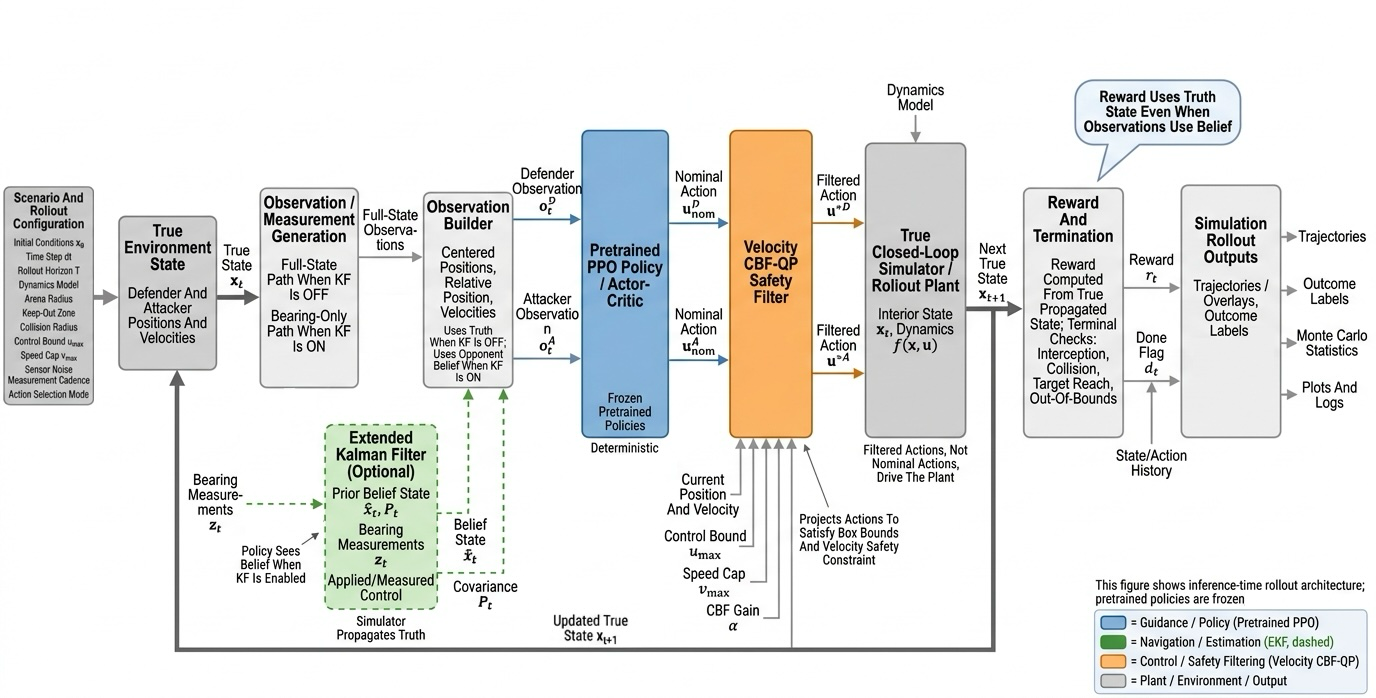
\includegraphics[width=1.0\linewidth]{Figures/Inference_Flattened.png}
    \caption{Diagram showing the inference described in algorithm \ref{alg:actuation_interface}}
    \label{fig:Inference_Flowchart}
\end{figure}


